\documentclass[10pt,landscape]{article}
\usepackage{multicol}
\usepackage{calc}
\usepackage{ifthen}
\usepackage[landscape]{geometry}
\usepackage{amsmath,amsthm,amsfonts,amssymb}
\usepackage{color,graphicx,overpic}
\usepackage{bm}
\usepackage{hyperref}



% This sets page margins to .5 inch if using letter paper, and to 1cm
% if using A4 paper. (This probably isn't strictly necessary.)
% If using another size paper, use default 1cm margins.
\ifthenelse{\lengthtest { \paperwidth = 11in}}
    { \geometry{top=1cm,left=1cm,right=1cm,bottom=1cm} }
    {\ifthenelse{ \lengthtest{ \paperwidth = 297mm}}
        {\geometry{top=1cm,left=1cm,right=1cm,bottom=1cm} }
        {\geometry{top=1cm,left=1cm,right=1cm,bottom=1cm} }
    }

% Turn off header and footer
\pagestyle{empty}

% Redefine section commands to use less space
\makeatletter
\renewcommand{\section}{\@startsection{section}{1}{0mm}%
                                {-1ex plus -.5ex minus -.2ex}%
                                {0.5ex plus .2ex}%x
                                {\normalfont\large\bfseries}}
\renewcommand{\subsection}{\@startsection{subsection}{2}{0mm}%
                                {-1explus -.5ex minus -.2ex}%
                                {0.5ex plus .2ex}%
                                {\normalfont\normalsize\bfseries}}
\renewcommand{\subsubsection}{\@startsection{subsubsection}{3}{0mm}%
                                {-1ex plus -.5ex minus -.2ex}%
                                {1ex plus .2ex}%
                                {\normalfont\small\bfseries}}
\makeatother
\newenvironment{lsmallmatrix}
{\left|\begin{smallmatrix}}
	{\end{smallmatrix}\right|}

\newcommand{\dx}{\mathrm{d}x}
\newcommand{\cd}{\overset{d}{\to}}
\newcommand{\cp}{\overset{p}{\to}}
\newcommand{\B}{\beta}
\newcommand{\e}{\epsilon}
\newcommand{\limn}{\lim_{n\to \infty}}
\newcommand{\lm}{\lambda}
\newcommand{\sg}{\sigma}
\newcommand{\hb}{\hat{\beta}}
\newcommand{\sumn}{\sum_{i=1}^{n}}
\newcommand{\hth}{\hat{\theta}}
\newcommand{\lra}{\Leftrightarrow}
\newcommand{\prodn}{\prod_{i=1}^{n}}
\allowdisplaybreaks
% Define BibTeX command
\def\BibTeX{{\rm B\kern-.05em{\sc i\kern-.025em b}\kern-.08em
    T\kern-.1667em\lower.7ex\hbox{E}\kern-.125emX}}

% Don't print section numbers
\setcounter{secnumdepth}{0}


\setlength{\parindent}{0pt}
\setlength{\parskip}{0pt plus 0.5ex}

%My Environments
\newtheorem{example}[section]{Example}
% -----------------------------------------------------------------------

\begin{document}

\raggedright
\footnotesize
\begin{multicols*}{4}
\setlength{\premulticols}{1pt}
\setlength{\postmulticols}{1pt}
\setlength{\multicolsep}{1pt}
\setlength{\columnsep}{2pt}

% multicol parameters
% These lengths are set only within the two main columns
\setlength{\columnseprule}{.25pt}
\setlength{\premulticols}{.25pt}
\setlength{\postmulticols}{.25pt}
\setlength{\multicolsep}{.25pt}
\setlength{\columnsep}{.25pt}
\textbf{SS and Est params}\\
 Corrected overall test compares full mod to intercept only mod. $H_0:\B_1=\cdots=0$\\
$SSH_{1x1}=(\hth-\theta_0)^{'}M^{-1}(\hth-\theta_0)$\\
$SSE=(y-\hat{y})^{'}(y-\hat{y})=y^{'}[I-H]y$\\
$\hb=(X^{'}X)^{-1}X^{'}y$ full rank\\
$H=X(X^{'}X)^{-1}X^{'}$ $rank(X)$\\
$Hy=\hat{y}$\quad
$M=C(X^{'}X)^{-1}C^{'}$\\
$\hat{y}=X\hb=Hy$ pred values\\
$\hat{\epsilon}=y-\hat{y}=y-Hy=(1-Hy)$\\\
$\hat{Var}(\hb)=\hat{\sg^2}(X^{'}X)^{-1}$ \\
$\hat{Var}(\hth)=\hat{\sg^2}(C(X^{'}X)^{-1}C^{'})$\quad $\hth=C\hb$\\
Use MSE for $\hat{\sg^2}$, use diag\\
$se=\sqrt{\hat{Var}}$\quad
$MS*=SS*/DF*$\\
$F=MST/MSE$\quad
$df_{total}=n-1$\\
t-value$=\hb/se$\quad
p-value$=F(df_{model},df_{error})$\\
95\% CI  $\hth\pm 1.96\sqrt{MSE(M)}$\\
F-Test$=\dfrac{(\hth-\theta_0)^{'}M^{-1}(\hth-\theta_0)/a}{\hat{\sg^2}}$ $a=rank(C)$\\
\textbf{Matrix}\\
$(X_{n\times p})^{'}(X_{n \times p})\hb=(X_{n\times p})^{'}y_{n\times 1}$ \\
$(AB)^{'}=B^{'}A^{'}$\quad
$A^{-1}A=AA^{-1}=I$\\
$(AB)^{-1}=B^{-1}A^{-1}$\quad
$(A^{'})^{-1}=(A^{-1})^{'}$\\
$|A^{-1}|=\dfrac{1}{|A|}$\quad
$\dfrac{1}{|A|}
\begin{lsmallmatrix}
a_{22}&-a_{12}\\
-a_{21}& a_{11}
\end{lsmallmatrix}$\\
det(inv)=inv(det)\quad
evector $Ax=\lm x$\quad
e val=$\lm$\\
char eqn $(|A-\lm I|=0)
=det\begin{lsmallmatrix}
a_{11}-\lm & a_{12}\\
a_{21} & a_{22}-\lm
\end{lsmallmatrix}$\\
full rank $\lra$ no $\lm=0$\quad
det=0  $\lra$ $\geq 1$ $\lm=0$\\
posdef $\lra$ diagval$>0$,
det all UL sq submat $>0$\\
semiposdef same but $\geq0$\\
cov mats are nonneg def\\
X full rank for $\hb$ unique\\
posdef if $min(\lm_i)>0$\\
E(rand mat)=mat of E\\
$Cov(Y)=E[(Y-\mu)(Y-\mu)^{'}]=\bm{\Sigma}$\\
$\begin{lsmallmatrix}
	\sigma_{11}&\sigma_{12}&\cdots& \sg_{1n}\\
	\sg_{21}& \vdots & \vdots & \vdots\\
	\vdots & \vdots & \vdots & \vdots\\
	\sg_{n1} &\cdots & \cdots& \sg_{nn} 
\end{lsmallmatrix}$\\
where $\sg_{ij}=E[(Y_i-\mu_i)(Y_j-\mu_j)^{'}]$\\
$Cov(AY+b)=A Cov(Y)A^{'}=A\Sigma A^{'}$
$Cov(W,Y)=E[(W-\gamma)(Y-\mu)^{'}]$\\
\textbf{MVN}
$\Sigma$ pos def\\
1) \textbf{lin trans} of mvn yields  mvn.\\
	If $X\sim N_n(\mu,\Sigma)$ and $Y=AX+b$\\
	with $A_{r\times n}$  matrix of constants and $\bm{b}_{r \times 1}$ vector of constants.\\
	Then $Y\sim N_r(A\mu+b,A\Sigma A^{'})$\\
	2) \textbf{lin combin} of ind mvns is mvn\\
	$X_1,\dots,X_k$ iid $X_i\sim N_n(\mu_i,\Sigma_i)$\\
	Let $Y=a_1X_1+\dots+a_kX_k$\\
	Then $Y\sim N(\mu^*,\Sigma^*)$ where $\mu^{*}=\sum_{i=1}^{k}a_i\mu_i$ and $\Sigma^*=\sum_{i=1}^{k}a_i^2\Sigma_i$\\
	3) \textbf{Marginals} of mvn are mvn\\
	If $X\sim N_n(\mu,\Sigma)$\\
	Partition:
	$X={X_1 \choose X_2}$ where $X_1$ is $r\times 1$ and $X_2$ is $(n-r)\times 1$\\
	$\mu={\mu_1\choose \mu_2}$ where $\mu_1$ is $r\times 1$ and $\mu_2$ is $(n-r)\times 1$\\
	$\Sigma=
	\begin{lsmallmatrix}
	\Sigma_{11}&\Sigma_{12}\\
	\Sigma_{21}&\Sigma_{22}
	\end{lsmallmatrix}$\\
	where $\Sigma_{11}$ is $r\times r$, $\Sigma_{21}$ is $(n-r)\times r$ and $\Sigma_{22}$ is $(n-r)\times (n-r)$\\
	Marginals:
	$X_1\sim N_r(\mu_1,\Sigma_{11})$\\ 
 $X_2\sim N_{(n-r)}(\mu_2,\Sigma_{22})$\\
4) \textbf{Conditionals} of mvn are mvn.\\
	Suppose $X\sim N_n(\mu,\Sigma)$\\
Partition same way\\
	$X_1|X_2=x_2\sim N_r(\mu_1+\Sigma_{12}\Sigma_{22}^{-1}(x_2-\mu_2),\Sigma^*)$\\
	where $\Sigma^*=\Sigma_{11}-\Sigma_{12}\Sigma_{22}^{-1}\Sigma_{21}$\\
\textbf{Estimable}\\
A (linear) function of the parameters that is identically equal to some linear function of the expected value of the vector of observations, $\bm{y}$\\
A scalar parameter,
	$\theta_i=\bm{C}_{1xp}\bm{\B}_{px1}$ is estimable $\lra \bm{C}_{1xp}\bm{\B}_{px1}=\bm{t^{'}}_{1xn}E(\bm{y}_{nx1})$
	for $\bm{t}$ a vector of constants\\
For a vector we need:
	$\bm{\theta}_{ax1}=\bm{T}_{axn}E(\bm{y}_{nx1})$\\
There always exists $r=rank(\bm{X})$ distinct and estimable parameters\\
These are not necessarily elements of $\bm{\B}$ but may be linear combinations of elements\\
If $rank(\bm{X})=r=p$, then $\bm{\hb}$ exists (uniquely), 
	$\bm{\B}$ is estimable and any (nonzero) $\bm{C}$ gives estimable $\bm{\theta}$\\
	This is usually the case with continuous predictors unless some predictors are collinear\\
If $rank(\bm{X})=r<p$, $\bm{\B}$ is not estimable (although as many as $r$ elements may be), and for $\bm{\hat{\theta}}=\bm{C\B}$, we must check estimability.\\
To show a set of parameters:
$\bm{\theta}_{a\times 1}=\bm{C}_{a\times p}\bm{\B}_{p\times1}=\bm{T}_{a\times n}E(\bm{y}_{n\times 1})$ is estimable:\\
show that $\bm{C}_{a\times p}=\bm{T}_{a\times n}\bm{X}_{n \times p}$\\
Estimable $\bm{\hat{\theta}}$ shares the optimality of $\bm{\hb}$\\
\textbf{Testability}\\
Let $\bm{M}_{a\times a}=\bm{C(X^{'}X)^{-1}C^{'}}$\\
Define GLH testability as the (unique) existence of the LR test\\
$\bm{\theta}$ is testable $\lra$
$\bm{C}$ is full rank $a$ (no redundancies) and
$\bm{\theta}$ is estimable\\
Or equivalently
$\bm{M}$ is full rank $a$ and
$\bm{\theta}$ is estimable\\
If $\bm{X}$ is full rank then $\bm{\theta}$ is testable $\Leftrightarrow$\\
$\bm{C}$ is full rank $a$ or $\bm{M}$ is full rank a (because any $\bm{\theta}$ is estimable)\\
All linear model GLH tests correspond to comparing two models, the "full" model, $\bm{y}=\bm{X\B}+\bm{\epsilon}$ and a reduced model defined by constraints\\
For a single coefficient $\B_j$ we can test $H_0:\B_j=0$ if $\B_j$ is estimable\\
$t=\frac{\hb_j-0}{\sqrt{var(\hb_j)}}$\\
Obtain estimate $\hat{\sg}^2=MSE$\\
if know $\sigma^2$  then $t\sim N(0,1)$\\
if estimate $\sg^2$ from data then $t\sim t_{dfE}$\\
\textbf{Sum of Squares Decomp}\\
$USS(total)=y^{'}y=\sumn y_i^2$\\
$USS(model)=y^{'}X(X^{'}X)^{-1}X^{'}y$\\
$=y^{'}Hy=\sumn \hat{y}_i^2$\\
$USS(total)=USS(model)+SSE$\\
$CSS(total)=USS(total)-SSI$\\
$=\sumn(y_i-\bar{y})^2$\\
$CSS(total)=CSS(model)+SSE$\\
\textbf{R squared,Corr}\\
$R^2_{adj}=1-\frac{SSE/(n-r)}{CSS(Total)/(n-1)}$\\
 adjusted for the df. It will only increase on
adding a variable to the model if the variable reduces the mean square
for error\\
$\rho=Corr(X,Y)=\frac{Cov(x,y)}{\sqrt{var(x)var(y)}}$\\
estimate $\rho$ using pearsons coef of corr\\
$R=\frac{\sumn(X_i-\bar{X})Y_i-\bar{Y}}{\sqrt{(\sumn
(X_i-\bar{X})^2)(\sumn (Y_i-\bar{Y})^2)}}$\\
\textbf{Diagnostics}\\
Homogeniety violations seen in pattern of resids\\
Independence through logic of sampling scheme\\
Linearity examine pattern of resid\\
Existence finite sample\\
Gaussian: (box plot, histogram, test of norm dist) all of resid\\
R/P plot provides the most useful
diagnostic because predicted values capture all the information in predictors that is available as a linear combination of them\\
Outlier-value (of a predictor or a response) much larger in
abs than next nearest val\\
LS est rather sensitive to outliers\\
A leverage value depends only on X and measures how extreme the
ith observation is in terms of the predictor space. An observation with
high leverage has the potential to have great influence on the model fit.\\
Influence-Cooks D, DFBETAS, DFFITS\\
Cooks Distance- extent
parameter estimates would change if we deleted ith
observation from sample\\
Predictors in model collinear whenever columns of X contain
redundancy.\\
\textbf{Type I}: $SS(A)$ for A, $SS(B | A)$ for B,
$SS(AB | B, A)$ for interaction AB\\
Tests  ME of A, followed by the ME of B after the ME of A, followed by AB after the MEs. Not great with unbalanced data\\
\textbf{Type III}: $SS(A | B, AB)$ for A, $SS(B | A, AB)$ for B.
Tests for ME after other ME and interact. Good for sig interacts,
not great ME\\
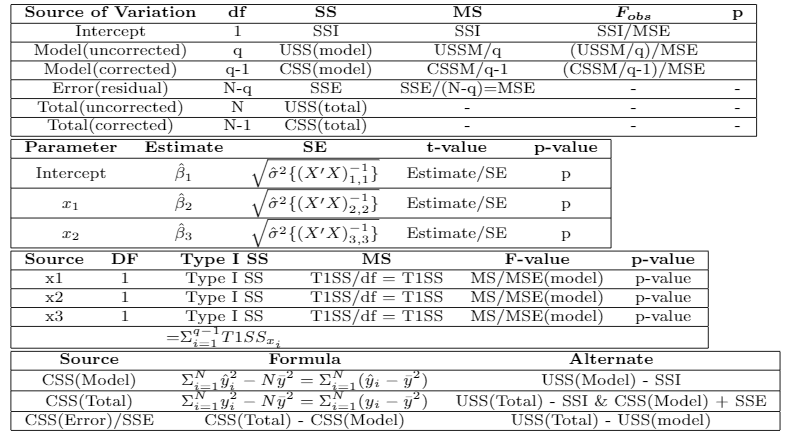
\includegraphics[scale=.535]{ss2.png}\\
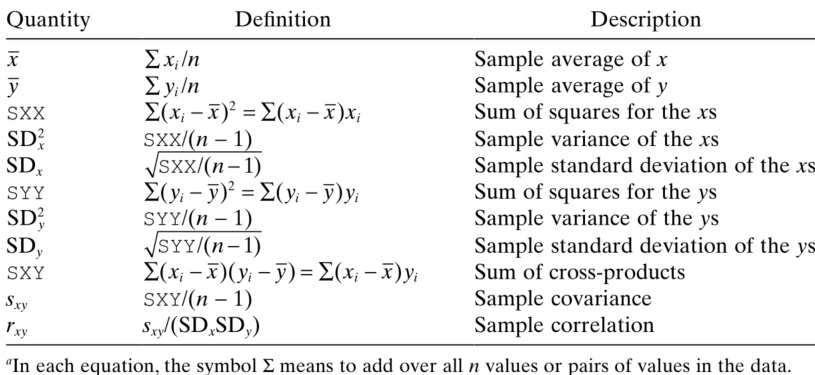
\includegraphics[scale=.3]{olsdefn.png}\\
$(X^{'}X)^{-1}=\begin{lsmallmatrix}
.308&-.06&-.017\\
-.06&-.025&-.004\\
-.017&-.004&.006
\end{lsmallmatrix}$ $X^{'}y=\begin{lsmallmatrix}
405\\1402\\2350
\end{lsmallmatrix}$\\
\scalebox{.7}{\begin{tabular}{l|l|l|l|l|l}
	\hline
	Source&DF  &SS  & MS  & Fval & $P>F$  \\
	\hline
	Model&2  &79  &239.5  &349.6& $<.001$ \\
	\hline
	Error& 97 & 11  & .113 &  \\
	\hline
	Ctotal&99  &90 &  & \\
	\hline
\end{tabular}}\\
\scalebox{.7}{\begin{tabular}{l|l|l|l|l|l}
	\hline
	param&est  &se  & tval  & $p>|t|$  \\
	\hline
	x0&.67  &.187  &3.58  &.009 \\
	\hline
	x1& 1.35 & .053  & 25.47&$<.001$ \\
	\hline
	x2&1.61  &.026 & 61.81 &$<.001$ \\
	\hline
\end{tabular}}\\
\textbf{2) c)} Test $H_0:\B_1=1$\\
t-test=$\frac{\hb_1-1}{se(\hb_1)}=6.6\sim t_{97}$ $6.6>1.96$ reject $H_0$\\
\textbf{d)} Test $H_0:\B_1=\B_2=1$\\
$B_1=1 \quad B_2=1$ \\
$C=\begin{lsmallmatrix}
0&1&0\\
0&0&1
\end{lsmallmatrix}$ $\theta_0=\begin{lsmallmatrix}
1\\
1
\end{lsmallmatrix}$ $H_0:C\theta=\theta_0$ $\hat{\theta}=\begin{lsmallmatrix}
1.35\\
1.61
\end{lsmallmatrix}$\\
calc M \quad calc $M^{-1}$\\
F-test=$\frac{43.83}{.113}=387.8\sim F_{2,97}$\\
\textbf{e)} 95\% CI of $\B_1+\B_2$ $(\theta)$\\
$\hth=\hb_1+\hb_2=2.96$ $C=[0,1,1]$\\
$se(\hth)=\hat{\sg}^2_{\hth}=\sqrt{.0026}$\\
$2.96\pm 1.96\sqrt{.0026}=[2.86,3.06]$\\
\textbf{f)} Transform $x_1$, $x_2$ to $z_1=x_1-2$, $z_2=x_2-4$\\
Refit with $y^*=\B_0^*+\B_1^*z_1+\B_2^*z_2$\\
$=(\B_0^*-2\B_1^*-4\B_2^*)+\B_1^*x_1+\B_2^*x_2$\\
$\B_0^*=\B_0^*+2\B_1^*+4\B_2^*=9.8$ $C=[1,2,4]$\\
$\sg^2=\hat{\sg}^2C(X^{'}X)^{-1}C^{-1}=.085$ $t=115.3$\\
\textbf{3) f)} is $H_0: \B_0-\B_2=0$ and $\B_1+2\B_2=2$ and $2\B_0+\B_1=2$ testable? Reduce to ETH?\\
$y=\begin{lsmallmatrix}
0\\2\\3\\6\\10
\end{lsmallmatrix}$ 
$X=\begin{lsmallmatrix}
1&6&11\\
1&7&13\\
1&8&15\\
1&9&17\\
1&11&21
\end{lsmallmatrix}$
$\B=\begin{lsmallmatrix}
\B_0 \\ \B_1 \\ \B_2
\end{lsmallmatrix}$\\
$C=\begin{lsmallmatrix}
1&0&-1\\
0&1&2\\
2&1&0
\end{lsmallmatrix}$reduces $\begin{lsmallmatrix}
1&0&-1\\
0&1&2\\
0&0&0
\end{lsmallmatrix}$ 2pivots $\theta_0=\begin{lsmallmatrix}
0\\2\\2
\end{lsmallmatrix}$\\
not FR, not testable, reduces to $C^*$ testable\\
$C^*=\begin{lsmallmatrix}
1&0&-1\\
0&1&2
\end{lsmallmatrix}$ $\theta^*_0=
\begin{lsmallmatrix}
0\\2
\end{lsmallmatrix}$ $H_0:\begin{lsmallmatrix}
\B_0-\B_2=0\\
\B_1+2\B_2=2
\end{lsmallmatrix}$\\

\end{multicols*} 
\end{document}